% Memory frontier (DATA plot) — RSS over the composite BDEC-CreGen prove run,
% M5 Pro 24 GB. Source: watcher trace risc0_cregen_composite_*/watch.log
% (peak 10.33 GB; plateaus 8-10 GB; never approaches the 24 GB wall -> the prior
% succinct failure was NOT memory). Shows the headroom that proves "not OOM".
% Downsampled, representative points (elapsed minutes, RSS GB).
% Compile: pdflatex memory_frontier.tex
\documentclass[border=4pt]{standalone}
\usepackage{newtxtext,newtxmath}
\usepackage{pgfplots}
\pgfplotsset{compat=1.18}
\definecolor{accent}{RGB}{210,120,30}
\begin{document}
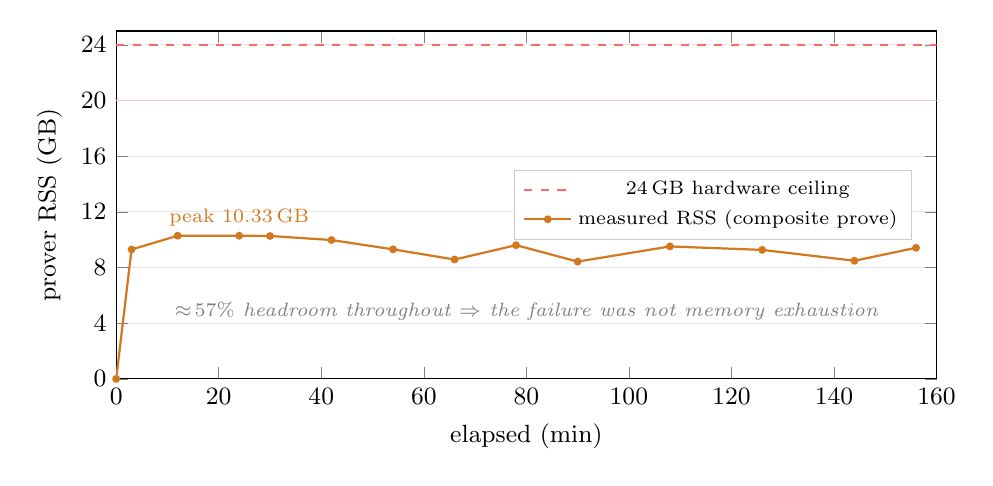
\begin{tikzpicture}
\begin{axis}[
  width=12cm, height=6cm,
  xlabel={elapsed (min)}, ylabel={prover RSS (GB)},
  ymin=0, ymax=25, xmin=0, xmax=160,
  ytick={0,4,8,12,16,20,24},
  ymajorgrids, grid style={gray!20},
  font=\small,
  legend style={at={(0.97,0.5)},anchor=east,font=\scriptsize,draw=gray!40},
]
% the 24 GB hardware ceiling
\addplot[red!60,dashed,thick,domain=0:160] {24};
\addlegendentry{24\,GB hardware ceiling}
% jetsam-pressure band (~20 GB, where OOM actually bites)
\addplot[red!25,domain=0:160,forget plot] {20};
% measured RSS trace (downsampled representative points, GB vs elapsed-min)
\addplot[accent,thick,mark=*,mark size=1pt] coordinates {
  (0,0.0) (3,9.3) (12,10.29) (24,10.29) (30,10.27) (42,9.98)
  (54,9.31) (66,8.58) (78,9.61) (90,8.43) (108,9.52) (126,9.27)
  (144,8.49) (156,9.42)
};
\addlegendentry{measured RSS (composite prove)}
% peak annotation
\node[font=\scriptsize,accent,anchor=south] at (axis cs:24,10.29) {peak $10.33$\,GB};
\node[font=\scriptsize\itshape,gray,anchor=north] at (axis cs:80,6.2)
  {$\approx\!57\%$ headroom throughout $\Rightarrow$ the failure was not memory exhaustion};
\end{axis}
\end{tikzpicture}
\end{document}
